\documentclass{report}
% PACKAGES %
\usepackage[english]{} % Sets the language
\usepackage[margin=2cm]{geometry} % Sets the margin size
\usepackage{graphicx} % Enhanced package for including graphics/figures
\usepackage{float} % Allows figures and tables to be floats
\usepackage{amsmath} % Enhanced math package prepared by the American Mathematical Society
\usepackage{amssymb} % AMS symbols package
\usepackage{bm} % Allows you to use \bm{} to make any symbol bold
\usepackage{verbatim} % Allows you to include code snippets
\usepackage{setspace} % Allows you to change the spacing between lines at different points in the document
\usepackage{parskip} % Allows you alter the spacing between paragraphs
\usepackage{multicol} % Allows text division into multiple columns
\usepackage{units} % Allows fractions to be expressed diagonally instead of vertically
\usepackage{booktabs,multirow,multirow} % Gives extra table functionality

\usepackage{rotating} % Allows tables to be rotated

\newcommand{\tab}{\-\hspace{1.5cm}}

% Set path to figure image files
\graphicspath{ {"C:/Users/Mitch/Documents/Cal/2 - 2017 Spring/COMPSCI 289A - Intro to Machine Learning/HW01/Figures/"} }

\begin{document}
{\bf {\large {COMPSCI 289A} Homework {1} \hfill {Mitchell Negus\\1/30/2017}}}\\\\
*Note: Code was worked on independently

%%%%%%%%%%%%%%%%%%%%%%%%%%%%%%%%%% PROBLEM 1 %%%%%%%%%%%%%%%%%%%%%%%%%%%%%%%%%%
\section*{Problem 1}

Data was partitioned as specified (10,000 validation images for MNIST, 20\% as validation samples for spam, and 5,000 validation images for CIFAR-10). 
See code, provided in the appendix, for evidence. Partitioning was accomplished by calling the partition function defined in HW01\_utils.py module.

\vspace{1.5cm}

%%%%%%%%%%%%%%%%%%%%%%%%%%%%%%%%%% PROBLEM 2 %%%%%%%%%%%%%%%%%%%%%%%%%%%%%%%%%%
\section*{Problem 2}

The linear SVM was trained on all three datasets. The score (accuracy) of the method was calculated for a range of samples. For each data set--MNIST, spam, and CIFAR-10--the error (error = 1-accuracy) is plotted as a function of $N$ samples used for training.

\vspace{0.5cm}
\textbf{MNIST}

Accuracy of MNIST training for 100, 200, 500, 1,000, 2,000, 5,000, and 10,000 training samples.

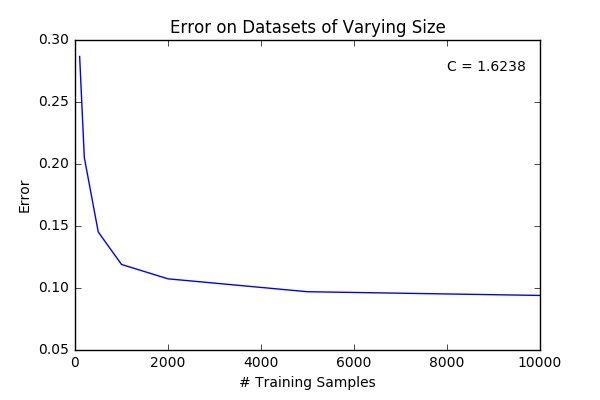
\includegraphics[width = 10cm]{MNIST_SampleAcc}

\newpage

\textbf{Spam}

Accuracy of spam/ham training for 100, 200, 500, 1,000, 2,000, and all (4,132) training samples.

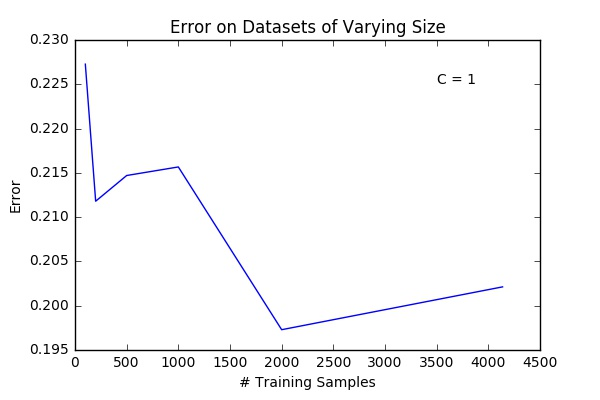
\includegraphics[width = 10cm]{spam_SampleAcc}

\vspace{0.5cm}
\textbf{CIFAR-10}

Accuracy of CIFAR-10 training for 100, 200, 500, 1,000, 2,000, and 5,000 training samples.

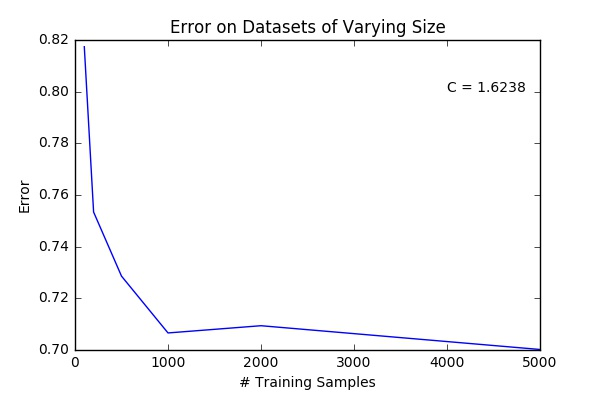
\includegraphics[width = 10cm]{CIFAR10_SampleAcc}	



%%%%%%%%%%%%%%%%%%%%%%%%%%%%%%%%%% PROBLEM 3 %%%%%%%%%%%%%%%%%%%%%%%%%%%%%%%%%%
\section*{Problem 3}

For the MNIST data set, the best value of $C$ was found to be $7.84759970351\times10^{-7}$, giving an accuracy of 92.98\%. All accuracies for a range of C values (all trained on 10,000 samples) are given below.

\-\\
\textbf{10,000 samples}\\
\textbf{C} \tab\tab \textbf{Accuracy}\\
1.0000E-08 \tab 0.8935\\
4.2813E-08 \tab 0.9147\\
1.8330E-07 \tab 0.9255\\
\textbf{7.8476E-07} \tab \textbf{0.9298}\\
3.3598E-06 \tab 0.9229\\
1.4384E-05 \tab 0.9118\\
6.1585E-05 \tab 0.9071\\
2.6367E-04 \tab 0.906\\
0.0011288 \tab 0.906\\
0.0048329 \tab 0.906\\
0.0206914 \tab 0.906\\
0.0885867 \tab 0.906\\
0.3792690 \tab 0.906\\
1.6237767 \tab 0.906\\
6.9519280 \tab 0.906\\
29.763514 \tab 0.906\\
127.42750 \tab 0.906\\
545.55948 \tab 0.906\\
2335.7215 \tab 0.906\\
10000.0 \tab\;\; 0.906\\

Full results for all sample counts are provided in the appendix.


%%%%%%%%%%%%%%%%%%%%%%%%%%%%%%%%%% PROBLEM 4 %%%%%%%%%%%%%%%%%%%%%%%%%%%%%%%%%%
\section*{Problem 4}

For the spam/ham data sets, best value of $C$ was found to be 100, giving an accuracy of 80.75\%. This value was found using a K-Fold Cross-Validation scheme where $k=5$. Below are all accuracies for a range of C values when the SVM was trained on 2,000 samples.

\-\\
\textbf{2,000 samples}\\
\textbf{C} \tab\tab \textbf{Accuracy}\\
1.0000E-08 \tab 0.710058\\
3.3598E-08 \tab 0.710058\\
1.1288E-07 \tab 0.710058\\
3.7927E-07 \tab 0.710058\\
1.2743E-06 \tab 0.710058\\
4.2813E-06 \tab 0.710058\\
1.4384E-05 \tab 0.710058\\
4.8329E-05 \tab 0.710058\\
0.00016238 \tab 0.717215\\
0.00054556 \tab 0.734429\\
0.00183298 \tab 0.750097\\
0.00615848 \tab 0.768279\\
0.02069138 \tab 0.779304\\
0.06951928 \tab 0.793617\\
0.23357215 \tab 0.8\\
0.78475997 \tab 0.802515\\
2.63665090 \tab 0.804836\\
8.85866790 \tab 0.805029\\
29.7635144 \tab 0.807350\\
\textbf{100.0} \hspace{0.7cm}\tab \textbf{0.807544}


%%%%%%%%%%%%%%%%%%%%%%%%%%%%%%%%%% PROBLEM 5 %%%%%%%%%%%%%%%%%%%%%%%%%%%%%%%%%%
\section*{Problem 5}

My Kaggle Leaderboard name: \textbf{mitch}\\
My Kaggle username: \textbf{mnegus}\\

\textbf{Kaggle Scores}:\\
MNIST:\; 0.93360 \tab\tab Spam:\; 0.84085 \\


\appendix

\huge{Appendix}\normalsize\\

Below are all accuracies tabulated for tested range of hyperparameter C for $N$ training samples.\\

% Table generated by Excel2LaTeX from sheet 'MNIST_Accuracies'
\begin{table}[htbp]
	\centering
	\small
	\caption{\textbf{MNIST}}
	\begin{tabular}{r||rrrrrrrrrrrrrrrrrrrr}
		\\
		$\bm{N}$\textbf{\textbackslash C} & 1E-08 & 4E-08 & 1.8E-07 & 7.8E-07 & 3.36E-06 & 1.44E-05 & 6.16E-05 & 0.000264 & 0.001129 & 0.004833 \\
		\toprule
		100   & 0.1119 & 0.2301 & 0.6438 & 0.7169 & 0.7133 & 0.7133 & 0.7133 & 0.7133 & 0.7133 & 0.7133 \\
		200   & 0.0963 & 0.425 & 0.7747 & 0.8005 & 0.7947 & 0.7947 & 0.7947 & 0.7947 & 0.7947 & 0.7947 \\
		500   & 0.3171 & 0.7527 & 0.865 & 0.8635 & 0.8552 & 0.8548 & 0.8548 & 0.8548 & 0.8548 & 0.8548 \\
		1000  & 0.5782 & 0.85  & 0.8867 & 0.8909 & 0.8815 & 0.881 & 0.881 & 0.881 & 0.881 & 0.881 \\
		2000  & 0.7981 & 0.8824 & 0.9043 & 0.9086 & 0.895 & 0.8926 & 0.8926 & 0.8926 & 0.8926 & 0.8926 \\
		5000  & 0.8721 & 0.9038 & 0.9183 & 0.9202 & 0.9135 & 0.9041 & 0.903 & 0.903 & 0.903 & 0.903 \\
		10000 & 0.8935 & 0.9147 & 0.9255 & 0.9298 & 0.9229 & 0.9118 & 0.9071 & 0.906 & 0.906 & 0.906 \\
		\midrule
		\midrule
		$\bm{N}$\textbf{\textbackslash C} & 0.020691 & 0.088587 & 0.379269 & 1.623777 & 6.951928 & 29.76351 & 127.4275 & 545.5595 & 2335.721 & 10000 \\
		\toprule
		100   & 0.7133 & 0.7133 & 0.7133 & 0.7133 & 0.7133 & 0.7133 & 0.7133 & 0.7133 & 0.7133 & 0.7133 \\
		200   & 0.7947 & 0.7947 & 0.7947 & 0.7947 & 0.7947 & 0.7947 & 0.7947 & 0.7947 & 0.7947 & 0.7947 \\
		500   & 0.8548 & 0.8548 & 0.8548 & 0.8548 & 0.8548 & 0.8548 & 0.8548 & 0.8548 & 0.8548 & 0.8548 \\
		1000  & 0.881 & 0.881 & 0.881 & 0.881 & 0.881 & 0.881 & 0.881 & 0.881 & 0.881 & 0.881 \\
		2000  & 0.8926 & 0.8926 & 0.8926 & 0.8926 & 0.8926 & 0.8926 & 0.8926 & 0.8926 & 0.8926 & 0.8926 \\
		5000  & 0.903 & 0.903 & 0.903 & 0.903 & 0.903 & 0.903 & 0.903 & 0.903 & 0.903 & 0.903 \\
		10000 & 0.906 & 0.906 & 0.906 & 0.906 & 0.906 & 0.906 & 0.906 & 0.906 & 0.906 & 0.906 \\
		
		\\
	\end{tabular}%
	\label{tab:addlabel}%
\end{table}%

% Table generated by Excel2LaTeX from sheet 'spam_Accuracies'
\begin{table}[htbp]
	\centering
	\small
	\caption{\textbf{Spam}}
	\begin{tabular}{r||rrrrrrrrrrrrrrrrrrrr}
		\\
		$\bm{N}$\textbf{\textbackslash C} & 1E-08 & 3E-08 & 1.1E-07 & 3.8E-07 & 1.27E-06 & 4.28E-06 & 1.44E-05 & 4.83E-05 & 0.000162 & 0.000546 \\
		\toprule
		100   & 0.710058 & 0.710058 & 0.710058 & 0.710058 & 0.710058 & 0.710058 & 0.710058 & 0.709865 & 0.710445 & 0.710638 \\
		200   & 0.710058 & 0.710058 & 0.710058 & 0.710058 & 0.710058 & 0.710058 & 0.710058 & 0.710058 & 0.710251 & 0.711025 \\
		500   & 0.710058 & 0.710058 & 0.710058 & 0.710058 & 0.710058 & 0.710058 & 0.710058 & 0.710058 & 0.710058 & 0.713926 \\
		1000  & 0.710058 & 0.710058 & 0.710058 & 0.710058 & 0.710058 & 0.710058 & 0.710058 & 0.710058 & 0.711412 & 0.725725 \\
		2000  & 0.710058 & 0.710058 & 0.710058 & 0.710058 & 0.710058 & 0.710058 & 0.710058 & 0.710058 & 0.717215 & 0.734429 \\
		4138  & 0.710058 & 0.710058 & 0.710058 & 0.710058 & 0.710058 & 0.710058 & 0.710058 & 0.712186 & 0.725338 & 0.743327 \\
		\midrule
		\midrule
		$\bm{N}$\textbf{\textbackslash C} & 0.001833 & 0.006158 & 0.020691 & 0.069519 & 0.233572 & 0.78476 & 2.636651 & 8.858668 & 29.76351 & 100 \\
		\toprule
		100   & 0.711605 & 0.716828 & 0.728433 & 0.74236 & 0.754932 & 0.770406 & 0.777756 & 0.786074 & 0.775629 & 0.781044 \\
		200   & 0.716441 & 0.730174 & 0.745261 & 0.758801 & 0.767892 & 0.782592 & 0.789555 & 0.798066 & 0.792456 & 0.786847 \\
		500   & 0.731141 & 0.745261 & 0.763636 & 0.77176 & 0.783172 & 0.791876 & 0.793424 & 0.793037 & 0.792456 & 0.792456 \\
		1000  & 0.741199 & 0.761896 & 0.7706 & 0.784139 & 0.790135 & 0.792843 & 0.797099 & 0.798646 & 0.79942 & 0.798453 \\
		2000  & 0.750097 & 0.768279 & 0.779304 & 0.793617 & 0.8   & 0.802515 & 0.804836 & 0.805029 & 0.80735 & 0.807544 \\
		4138  & 0.763056 & 0.774855 & 0.789362 & 0.794971 & 0.79942 & 0.801354 & 0.802128 & 0.802901 & 0.802708 & 0.802515 \\
		
		\\
	\end{tabular}%
	\label{tab:addlabel}%
\end{table}%


% Table generated by Excel2LaTeX from sheet 'CIFAR_Accuracies'
\begin{table}[htbp]
	\centering
	\small
	\caption{\textbf{CIFAR-10}}
	\begin{tabular}{r||rrrrrrrrrrrrrrrrrrrr}
		\\
		$\bm{N}$\textbf{\textbackslash C} & 1E-08 & 4E-08 & 1.8E-07 & 7.8E-07 & 3.36E-06 & 1.44E-05 & 6.16E-05 & 0.000264 & 0.001129 & 0.004833 \\
		\toprule
		100   & 0.111 & 0.1658 & 0.1834 & 0.1838 & 0.1826 & 0.1826 & 0.1826 & 0.1826 & 0.1826 & 0.1826 \\
		200   & 0.1026 & 0.2272 & 0.2622 & 0.2466 & 0.2466 & 0.2466 & 0.2466 & 0.2466 & 0.2466 & 0.2466 \\
		500   & 0.2202 & 0.295 & 0.3008 & 0.2842 & 0.2708 & 0.2714 & 0.2714 & 0.2714 & 0.2714 & 0.2714 \\
		1000  & 0.2632 & 0.3164 & 0.3306 & 0.3148 & 0.2934 & 0.2934 & 0.2934 & 0.2934 & 0.2934 & 0.2934 \\
		2000  & 0.3   & 0.3476 & 0.345 & 0.321 & 0.3016 & 0.291 & 0.2906 & 0.2906 & 0.2906 & 0.2906 \\
		5000  & 0.353 & 0.3736 & 0.3752 & 0.3518 & 0.3216 & 0.3066 & 0.2992 & 0.2998 & 0.2998 & 0.2998 \\
		\midrule
		\midrule
		$\bm{N}$\textbf{\textbackslash C} & 0.020691 & 0.088587 & 0.379269 & 1.623777 & 6.951928 & 29.76351 & 127.4275 & 545.5595 & 2335.721 & 10000 \\
		\toprule
		100   & 0.1826 & 0.1826 & 0.1826 & 0.1826 & 0.1826 & 0.1826 & 0.1826 & 0.1826 & 0.1826 & 0.1826 \\
		200   & 0.2466 & 0.2466 & 0.2466 & 0.2466 & 0.2466 & 0.2466 & 0.2466 & 0.2466 & 0.2466 & 0.2466 \\
		500   & 0.2714 & 0.2714 & 0.2714 & 0.2714 & 0.2714 & 0.2714 & 0.2714 & 0.2714 & 0.2714 & 0.2714 \\
		1000  & 0.2934 & 0.2934 & 0.2934 & 0.2934 & 0.2934 & 0.2934 & 0.2934 & 0.2934 & 0.2934 & 0.2934 \\
		2000  & 0.2906 & 0.2906 & 0.2906 & 0.2906 & 0.2906 & 0.2906 & 0.2906 & 0.2906 & 0.2906 & 0.2906 \\
		5000  & 0.2998 & 0.2998 & 0.2998 & 0.2998 & 0.2998 & 0.2998 & 0.2998 & 0.2998 & 0.2998 & 0.2998 \\
		
		\\
	\end{tabular}%
	\label{tab:addlabel}%
\end{table}%

\vspace{25cm}
Included on the following pages is the code used for this project: namely the 3 Jupyter notebooks and 2 python modules:
\end{document}

